\documentclass[sigconf]{acmart}

%% Remove ACM reference format for draft
\settopmatter{printacmref=false}
\renewcommand\footnotetextcopyrightpermission[1]{}
\pagestyle{plain}

\usepackage{booktabs}
\usepackage{amsmath}
\usepackage{amssymb}
\usepackage{graphicx}
\usepackage{microtype}
\usepackage{xcolor}
\usepackage{tikz}
\usetikzlibrary{arrows.meta, positioning, shapes.geometric, fit, backgrounds, calc}
\usepackage{pifont}
\newcommand{\cmark}{\ding{51}}
\newcommand{\xmark}{\ding{55}}

%% ======================================================
%%  Paper metadata  — fill in before submission
%% ======================================================
\acmConference[SIGSPATIAL '26]{34th ACM SIGSPATIAL}{November 2026}{Atlanta, GA}
\acmYear{2026}
\copyrightyear{2026}

\begin{document}

%% -------------------------------------------------------
%%  Title
%% -------------------------------------------------------
% Title variants — send to Prof + Buddhi to choose:
%   (A) WJ-Native Autoencoder Compression for Efficient Polygon Similarity Search  [ACTIVE]
%   (B) Learning WJ-Preserving Autoencoder Embeddings for Efficient Polygon Retrieval
%   (C) Compact Autoencoder Compression for Efficient Weighted-Jaccard Polygon Search
\title{WJ-Native Autoencoder Compression for Efficient Polygon Similarity Search}

\author{Ruban Sampath}
\affiliation{%
  \institution{Univ. of Texas at San Antonio}
  \city{San Antonio}
  \country{USA}}
\email{ruban.s@utsa.edu}

\author{Buddhi Ashan M. K.}
\affiliation{%
  \institution{Univ. of Texas at San Antonio}
  \city{San Antonio}
  \country{USA}}
\email{buddhiashan.mallikakankanamalage@utsa.edu}

\author{Sushil K. Prasad}
\affiliation{%
  \institution{Univ. of Texas at San Antonio}
  \city{San Antonio}
  \country{USA}}
\email{sushil.prasad@utsa.edu}

\renewcommand{\shortauthors}{Sampath et al.}

%% -------------------------------------------------------
%%  Abstract
%% -------------------------------------------------------
\begin{abstract}
Similarity search over polygon datasets is a critical operation in spatial data
management, where Weighted Jaccard (WJ) captures area-based shape overlap.
ShapeToVec encodes polygons as 18{,}219-dimensional probability simplex vectors
enabling direct Hierarchical Navigable Small World (HNSW) retrieval, but the high
dimensionality imposes significant memory and query-time overhead.
We propose a learned \emph{autoencoder} compression framework that maps these vectors
to compact 512-dimensional simplex embeddings, enabling WJ-compatible HNSW indexing
with 36$\times$ smaller vectors.
Our encoder is trained with a WJ-native triplet loss, in-batch hard negative mining,
and false-negative filtering; a decoder adds a reconstruction objective that forces
the encoder to preserve fine-grained geometry beyond pairwise rank order.
Our autoencoder achieves R@10\,=\,0.711 and R@50\,=\,0.858 at 10{,}903 queries per
second (QPS) ---
78$\times$ higher throughput than brute-force ICWS (Improved Consistent Weighted
Sampling).
After Stage-2 exact-WJ reranking, R@10 exceeds 0.996 across all our variants.
Systematic ablations reveal that false-negative filtering and reconstruction are
complementary: without filtering, adding reconstruction causes conflicting gradients
that collapse recall to 0.510.
Scaling to the full 187k-polygon corpus, we find that ranking-based objectives no
longer outperform an untrained random projection. We close this gap by training the
encoder as a candidate \emph{filter} --- a non-saturating contrastive objective over
the broad neighbourhood --- which restores recall and yields a more navigable index.
This is, to our knowledge, the first learned WJ embedding to surpass random
projection on the recall--throughput frontier at scale: equal top-50 reranked recall
at $\sim$1.9$\times$ higher query throughput.
\end{abstract}

\keywords{polygon similarity search, weighted Jaccard, metric learning, approximate
nearest neighbor, probability simplex, autoencoder}

%%
%% ACM CCS concepts
%%
\begin{CCSXML}
<ccs2012>
  <concept>
    <concept_id>10002951.10003317.10003347.10003350</concept_id>
    <concept_desc>Information systems~Similarity search</concept_desc>
    <concept_significance>500</concept_significance>
  </concept>
  <concept>
    <concept_id>10002951.10003317.10003318</concept_id>
    <concept_desc>Information systems~Nearest-neighbor search</concept_desc>
    <concept_significance>500</concept_significance>
  </concept>
  <concept>
    <concept_id>10010147.10010257.10010293.10010294</concept_id>
    <concept_desc>Computing methodologies~Neural networks</concept_desc>
    <concept_significance>300</concept_significance>
  </concept>
  <concept>
    <concept_id>10002951.10003227.10003351.10003445</concept_id>
    <concept_desc>Information systems~Geographic information systems</concept_desc>
    <concept_significance>300</concept_significance>
  </concept>
</ccs2012>
\end{CCSXML}

\ccsdesc[500]{Information systems~Similarity search}
\ccsdesc[500]{Information systems~Nearest-neighbor search}
\ccsdesc[300]{Computing methodologies~Neural networks}
\ccsdesc[300]{Information systems~Geographic information systems}

\received{June 2026}

\maketitle

%% -------------------------------------------------------
%%  1. Introduction
%% -------------------------------------------------------
\section{Introduction}

Geospatial applications increasingly rely on large polygon datasets --- parks,
water bodies, parcel boundaries, and land-use regions --- where finding similar
shapes is essential for data deduplication, conflation, and spatial analytics.
Weighted Jaccard (WJ) similarity,
\begin{equation}
  WJ(\mathbf{a},\mathbf{b}) = \frac{\sum_i \min(a_i,b_i)}{\sum_i \max(a_i,b_i)},
  \quad \mathbf{a},\mathbf{b} \geq \mathbf{0},
  \label{eq:wj}
\end{equation}
captures area-weighted shape overlap and is the standard metric for this task.
A central obstacle in encoding such polygons is \emph{extreme area variability}:
in real-world GIS corpora, polygon areas span several orders of magnitude (e.g.\
a neighbourhood park versus a national forest). A uniform rasterisation grid
cannot serve both regimes --- a grid fine enough to resolve small polygons
explodes in dimensionality, while a grid coarse enough to be tractable leaves
small polygons occupying only a handful of cells, collapsing their shape
information into near-empty vectors. ShapeToVec~\cite{shape2vec} resolves this
with an adaptive \emph{quadtree} grid that recursively subdivides space where
polygon detail is concentrated, encoding each polygon as an 18{,}219-dimensional
probability-simplex vector whose WJ preserves area-weighted shape overlap across
all scales. Indexed directly with HNSW, ShapeToVec attains 97\% R@50 on corpora
up to 1.7M polygons. However, indexing such large vectors becomes increasingly
expensive as corpora grow; compressing them while preserving WJ structure
enables faster search and lower memory overhead at scale.

Classical Locality-Sensitive Hashing (LSH) methods such as Improved Consistent
Weighted Sampling (ICWS)~\cite{ioffe10} and ProbMinHash~\cite{probminhash20} produce
theoretically optimal WJ sketches but output integer codes that require brute-force
comparison, yielding 139\,QPS on our evaluation corpus.
PolyMinHash~\cite{polyminhash25} reduces candidates via LSH banding, yet remains
non-learned and cannot adapt to data distribution.
Learned hashing and metric learning methods~\cite{hashsurvey14,deephashsurvey22}
train neural networks to compress vectors for fast HNSW search, but exclusively
target Euclidean or Hamming spaces --- none produce WJ-compatible embeddings.

We address this gap. Our contributions are:
\begin{enumerate}
  \item \textbf{WJ-native embedding}: we constrain encoder outputs to the
    probability simplex via Rectified Linear Unit (ReLU)\,+\,L1-normalisation,
    so that WJ is directly computable between compressed embeddings and nmslib's
    \texttt{WeightedJaccard} HNSW space can be used without any post-processing.
  \item \textbf{MLP cosine triplet encoder (ours)}: we design a three-layer
    multi-layer perceptron (MLP) encoder trained with cosine triplet loss as a
    strong learned baseline, demonstrating that neural compression substantially
    outperforms Principal Component Analysis (PCA), Non-negative Matrix
    Factorization (NMF), and random projection on WJ retrieval
    (Table~\ref{tab:results}).
  \item \textbf{WJ triplet training with false-negative filtering}: we replace cosine
    similarity with WJ in the triplet loss and add ground-truth (GT) masking to
    prevent known GT neighbours from corrupting hard-negative gradients.
  \item \textbf{Autoencoder reconstruction improves WJ metric learning}: adding a
    decoder reconstruction objective improves Stage-1 R@50 by
    5.0\,percentage points (pp) over the triplet-only MLP, but \emph{only} when
    false-negative filtering is active --- without it, conflicting gradients collapse
    recall to 0.510.
  \item \textbf{Filter training scales where ranking does not}: on the full
    187k-polygon corpus, ranking objectives degrade to the level of an untrained
    random projection. Training the encoder as a candidate filter --- a
    non-saturating contrastive objective over the broad neighbourhood --- restores
    recall and produces a more navigable index, beating random projection by
    $\sim$1.9$\times$ in throughput at equal top-50 reranked recall
    (Sec.~\ref{sec:fullscale}).
\end{enumerate}

Figure~\ref{fig:pipeline} illustrates the full two-stage retrieval pipeline.

%% -------------------------------------------------------
%%  Architecture figure  (infographic style)
%% -------------------------------------------------------
\begin{figure*}[t]
\centering
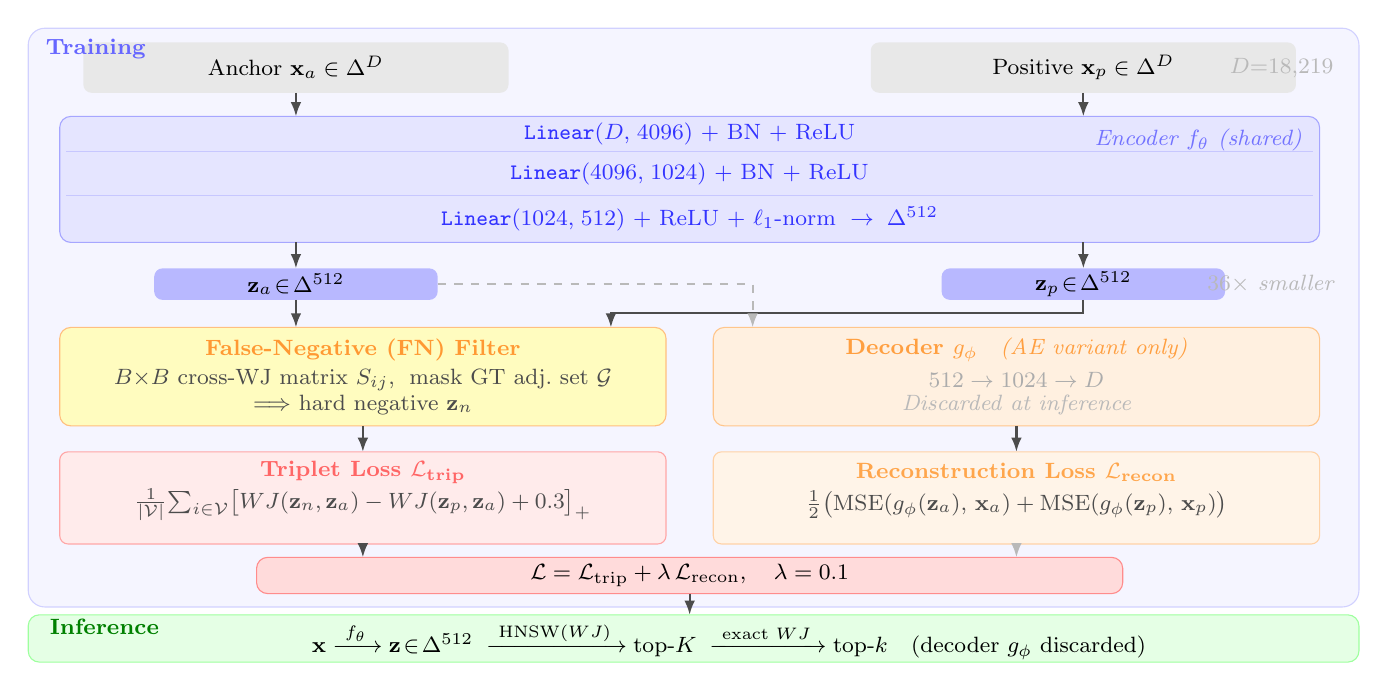
\begin{tikzpicture}[
  x=1cm, y=1cm,
  font=\footnotesize,
  arr/.style  = {-{Latex[length=1.8mm]}, thick, black!70},
  darr/.style = {-{Latex[length=1.8mm]}, thick, dashed, gray!55},
]

%% ── Row 0: inputs ─────────────────────────────────────────────────────────
\fill[gray!18, rounded corners=3pt] (0.3, 0.32) rectangle (5.7,-0.32);
\node at (3.0, 0) {Anchor $\mathbf{x}_a \in \Delta^{D}$};

\fill[gray!18, rounded corners=3pt] (10.3, 0.32) rectangle (15.7,-0.32);
\node at (13.0, 0) {Positive $\mathbf{x}_p \in \Delta^{D}$};

\node[font=\footnotesize\itshape, text=gray!55, anchor=east]
  at (16.3, 0) {$D{=}18{,}219$};

\draw[arr] (3.0,-0.32) -- (3.0,-0.62);
\draw[arr] (13.0,-0.32) -- (13.0,-0.62);

%% ── Row 1: encoder ─────────────────────────────────────────────────────────
\fill[blue!10, rounded corners=4pt] (0.0,-0.62) rectangle (16.0,-2.22);
\draw[blue!35, rounded corners=4pt] (0.0,-0.62) rectangle (16.0,-2.22);
\draw[blue!22] (0.08,-1.07) -- (15.92,-1.07);
\draw[blue!22] (0.08,-1.62) -- (15.92,-1.62);
\node[text=blue!80] at (8.0,-0.845)
  {\texttt{Linear}($D$,\;4096) + BN + ReLU};
\node[text=blue!80] at (8.0,-1.345)
  {\texttt{Linear}(4096,\;1024) + BN + ReLU};
\node[text=blue!80] at (8.0,-1.920)
  {\texttt{Linear}(1024,\;512) + ReLU + $\ell_1$-norm $\;\to\; \Delta^{512}$};
\node[font=\footnotesize\itshape, text=blue!55, anchor=north east]
  at (15.9,-0.65) {Encoder $f_\theta$ (shared)};

\draw[arr] (3.0,-2.22) -- (3.0,-2.55);
\draw[arr] (13.0,-2.22) -- (13.0,-2.55);

%% ── Row 2: compact embeddings ───────────────────────────────────────────────
\fill[blue!28, rounded corners=3pt] (1.2,-2.55) rectangle (4.8,-2.95);
\node at (3.0,-2.75) {$\mathbf{z}_a\!\in\!\Delta^{512}$};

\fill[blue!28, rounded corners=3pt] (11.2,-2.55) rectangle (14.8,-2.95);
\node at (13.0,-2.75) {$\mathbf{z}_p\!\in\!\Delta^{512}$};

\node[font=\footnotesize\itshape, text=gray!55, anchor=east]
  at (16.3,-2.75) {$36{\times}$ smaller};

%% ── Arrows to Row 3 ─────────────────────────────────────────────────────────
\draw[arr] (3.0,-2.95) -- (3.0,-3.30);
\draw[arr] (13.0,-2.95) -- ++(0,-0.17) -| (7.0,-3.30);
\draw[darr] (4.8,-2.75) -- (8.8,-2.75) -- (8.8,-3.30);

%% ── Row 3: FN filter (left) + Decoder (right) ──────────────────────────────
\fill[yellow!25, rounded corners=4pt] (0.0,-3.30) rectangle (7.7,-4.55);
\draw[orange!50, rounded corners=4pt] (0.0,-3.30) rectangle (7.7,-4.55);
\node[font=\footnotesize\bfseries, text=orange!80] at (3.85,-3.58)
  {False-Negative (FN) Filter};
\node[text=black!70] at (3.85,-3.97)
  {$B{\times}B$ cross-WJ matrix $S_{ij}$,\; mask GT adj.\ set $\mathcal{G}$};
\node[text=black!70] at (3.85,-4.28)
  {$\Longrightarrow$ hard negative $\mathbf{z}_n$};

\fill[orange!12, rounded corners=4pt] (8.3,-3.30) rectangle (16.0,-4.55);
\draw[orange!45, rounded corners=4pt] (8.3,-3.30) rectangle (16.0,-4.55);
\node[font=\footnotesize\bfseries, text=orange!75] at (12.15,-3.58)
  {Decoder $g_\phi$ \enspace {\normalfont\footnotesize\itshape(AE variant only)}};
\node[text=gray!65] at (12.15,-3.97) {$512 \to 1024 \to D$};
\node[font=\footnotesize\itshape, text=gray!55] at (12.15,-4.28)
  {Discarded at inference};

%% ── Arrows to Row 4 ─────────────────────────────────────────────────────────
\draw[arr] (3.85,-4.55) -- (3.85,-4.88);
\draw[arr] (12.15,-4.55) -- (12.15,-4.88);

%% ── Row 4: losses ───────────────────────────────────────────────────────────
\fill[red!8, rounded corners=3pt] (0.0,-4.88) rectangle (7.7,-6.05);
\draw[red!35, rounded corners=3pt] (0.0,-4.88) rectangle (7.7,-6.05);
\node[font=\footnotesize\bfseries, text=red!60] at (3.85,-5.14)
  {Triplet Loss $\mathcal{L}_{\text{trip}}$};
\node[text=black!70] at (3.85,-5.55)
  {$\frac{1}{|\mathcal{V}|}\!\sum_{i\in\mathcal{V}}
    \bigl[WJ(\mathbf{z}_n,\mathbf{z}_a) - WJ(\mathbf{z}_p,\mathbf{z}_a)+0.3\bigr]_+$};

\fill[orange!9, rounded corners=3pt] (8.3,-4.88) rectangle (16.0,-6.05);
\draw[orange!35, rounded corners=3pt] (8.3,-4.88) rectangle (16.0,-6.05);
\node[font=\footnotesize\bfseries, text=orange!70] at (12.15,-5.14)
  {Reconstruction Loss $\mathcal{L}_{\text{recon}}$};
\node[text=black!70] at (12.15,-5.55)
  {$\tfrac{1}{2}\bigl(\mathrm{MSE}(g_\phi(\mathbf{z}_a),\,\mathbf{x}_a)
    + \mathrm{MSE}(g_\phi(\mathbf{z}_p),\,\mathbf{x}_p)\bigr)$};

%% ── Row 5: combined loss ────────────────────────────────────────────────────
\fill[red!14, rounded corners=4pt] (2.5,-6.22) rectangle (13.5,-6.68);
\draw[red!45, rounded corners=4pt] (2.5,-6.22) rectangle (13.5,-6.68);
\node at (8.0,-6.45)
  {$\mathcal{L} = \mathcal{L}_{\text{trip}} + \lambda\,\mathcal{L}_{\text{recon}},
    \quad \lambda=0.1$};

\draw[arr]  (3.85,-6.05) -- (3.85,-6.22);
\draw[darr] (12.15,-6.05) -- (12.15,-6.22);

%% ── Training background ─────────────────────────────────────────────────────
\begin{scope}[on background layer]
  \fill[blue!4, rounded corners=6pt]
    (-0.4, 0.50) rectangle (16.5,-6.85);
  \draw[blue!18, rounded corners=6pt]
    (-0.4, 0.50) rectangle (16.5,-6.85);
\end{scope}
\node[font=\footnotesize\bfseries, text=blue!60, anchor=north west]
  at (-0.30, 0.48) {Training};

%% ── Inference strip ─────────────────────────────────────────────────────────
\fill[green!10, rounded corners=4pt]
  (-0.4,-6.95) rectangle (16.5,-7.55);
\draw[green!38, rounded corners=4pt]
  (-0.4,-6.95) rectangle (16.5,-7.55);
\node[font=\footnotesize\bfseries, text=green!50!black, anchor=west]
  at (-0.25,-7.10) {Inference};
\node at (8.5,-7.28)
  {$\mathbf{x}
    \xrightarrow{\;f_\theta\;}
    \mathbf{z}\!\in\!\Delta^{512}
    \;\xrightarrow{\;\mathrm{HNSW}(WJ)\;}
    \text{top-}K
    \;\xrightarrow{\;\text{exact }WJ\;}
    \text{top-}k$\quad(decoder $g_\phi$ discarded)};
\draw[arr] (8.0,-6.68) -- (8.0,-6.95);

\end{tikzpicture}
\caption{Training pipeline and two-stage inference.
  Anchor and positive are encoded by the shared encoder $f_\theta$
  ($36\times$ compression: $D{=}18{,}219 \to 512$).
  Hard negatives are mined from the in-batch cross-WJ matrix after
  masking GT neighbours (FN filter $\mathcal{G}$).
  The decoder $g_\phi$ (dashed; AE variant only) contributes
  $\mathcal{L}_{\text{recon}}$ and is discarded at inference.}
\label{fig:pipeline}
\end{figure*}

%% -------------------------------------------------------
%%  2. Related Work
%% -------------------------------------------------------
\section{Related Work}

\paragraph{Polygon representation and ShapeToVec.}
Representing polygons for similarity search requires encoding geometric structure
into a form amenable to efficient indexing.
Uniform-grid approaches assign each polygon a fixed-resolution rasterisation, but
they fail in the presence of extreme area variation: a fine grid sized for large
polygons leaves small polygons with nearly all-zero cells, collapsing their
geometric representation; a coarse grid discards fine detail for small shapes.
ShapeToVec~\cite{shape2vec} addresses this with an adaptive quadtree decomposition
that recursively subdivides cells according to polygon coverage, producing
18{,}219-dimensional probability simplex vectors whose WJ captures area-weighted
shape overlap across all scales.
Indexed directly with HNSW~\cite{hnsw20}, ShapeToVec achieves $\geq$97\% R@50 on
corpora up to 1.7M polygons; our work learns to compress these vectors to 512
dimensions while preserving their WJ structure.

\paragraph{WJ sketching.}
ICWS~\cite{ioffe10} generates 512-dimensional sketches where the expected number
of agreeing positions equals the WJ similarity, providing an unbiased estimator.
ProbMinHash~\cite{probminhash20} accelerates sketch generation by orders of
magnitude while preserving the same guarantee.
Both methods output integer codes incompatible with float-vector approximate nearest
neighbor (ANN) indexes, requiring brute-force or LSH-band search at query time.
PolyMinHash~\cite{polyminhash25} applies area-based MinHashing directly to polygon
geometry with LSH banding for candidate pruning, but is non-learned.

\paragraph{Learned hashing and metric learning.}
Learning-to-hash methods~\cite{hashsurvey14,deephashsurvey22} train networks to
map inputs to compact binary codes for Hamming-distance search.
Metric learning with triplet~\cite{hashsurvey14} or contrastive losses produces
real-valued embeddings for Euclidean/cosine ANN search.
Matryoshka Representation Learning~\cite{matryoshka22} trains nested prefix
embeddings for flexible truncation; designed for cosine space, it degrades on the
WJ-simplex task (Table~\ref{tab:results}).
NMF~\cite{nmf99} factorises the data matrix into non-negative components, yielding
simplex-compatible embeddings without labels but optimising reconstruction rather
than WJ retrieval.
None of the above methods target WJ as the native similarity metric.

%% -------------------------------------------------------
%%  3. Method
%% -------------------------------------------------------
\section{Method}

\subsection{Problem Formulation}

Given a corpus $\mathcal{D} = \{\mathbf{x}_i\}_{i=1}^N$ of ShapeToVec polygon
encodings $\mathbf{x}_i \in \Delta^D$ ($D = 18{,}219$) and a set of ground-truth
WJ nearest-neighbour pairs $\mathcal{P} \subset \mathcal{D} \times \mathcal{D}$,
our goal is to learn a compact encoder $f_\theta: \Delta^D \to \Delta^d$ ($d = 512$)
such that WJ similarity is preserved in the compressed space, enabling fast HNSW
retrieval with WJ as the index metric.

\subsection{Encoder Architecture}
\label{sec:arch}

The encoder $h_\theta$ is a three-layer MLP with Batch Normalization (BN) and
ReLU activations ($18{,}219 \to 4{,}096 \to 1{,}024 \to 512$, $\sim$80M
parameters). Three considerations dictate this design, each driven by the
structure of WJ and of the quadtree input rather than by convention.

\noindent\textbf{Why an MLP, not a Transformer or graph encoder.}
The neural polygon encoders common in the literature --- boundary Transformers,
vertex graph networks, and set encoders --- target cosine or Euclidean output
spaces and fail catastrophically when repurposed for WJ retrieval
($R@50<0.02$~\cite{sampath25}). Two mismatches explain this. First,
\emph{space mismatch}: an encoder trained under an L2 or cosine objective learns
a metric structure that is destroyed when its outputs are forced onto the WJ
simplex via ReLU\,+\,$\ell_1$-normalisation. Second, \emph{loss of global
structure}: sequence- and graph-based encoders aggregate \emph{local} context
(token windows, vertex hops), whereas WJ is a global statistic summed over all
$D$ dimensions that cannot be decomposed into local sub-computations. A plain
MLP trained \emph{natively} in WJ space avoids both.

\noindent\textbf{Global projection.}
Accordingly, the first layer is a single dense projection
$\mathbb{R}^{18{,}219}\!\to\!\mathbb{R}^{4{,}096}$ that mixes \emph{all} input
dimensions in one matrix multiply, so every pair of quadtree cells can interact
and the cross-dimension co-occurrence statistics WJ depends on are preserved.
This global mixing is why $\sim$75M of the $\sim$80M parameters reside in this
first layer.

\noindent\textbf{BatchNorm before ReLU.}
Quadtree rasterization yields extremely sparse vectors (mean $\sim$73\% zeros,
mean non-zero entry $\sim$$10^{-9}$), so pre-activation responses have near-zero
variance. Applying ReLU directly would suppress almost all activations and
produce a degenerate output whose pairwise WJ varies by $\sim$$10^{-4}$ --- too
little to rank candidates. Placing BN \emph{before} each ReLU re-centers and
rescales the activations first, guaranteeing a non-degenerate output distribution.

\subsection{Probability Simplex Output Constraint}

WJ (Eq.~\ref{eq:wj}) requires non-negative inputs. We enforce this with a final
simplex projection layer:
\begin{equation}
  f_\theta(\mathbf{x}) = \frac{\operatorname{ReLU}(h_\theta(\mathbf{x}))}
                              {\max\!\bigl(\|\operatorname{ReLU}(h_\theta(\mathbf{x}))\|_1,\;\epsilon\bigr)}.
  \label{eq:simplex}
\end{equation}
The output sequence BN\,$\to$\,ReLU\,$\to$\,$\ell_1$-norm is necessary and
sufficient for WJ compatibility: non-negativity makes the element-wise
$\min$/$\max$ meaningful, and $\ell_1$-normalisation places every embedding on
the probability simplex $\Delta^{512}$ so the $\min$/$\max$ ratio is computed at
a comparable scale. Together this (i)~makes
$WJ(f_\theta(\mathbf{x}), f_\theta(\mathbf{y}))$ well-defined for any input pair,
and (ii)~enables direct use of nmslib's \texttt{WeightedJaccard} HNSW space
without post-processing.

\subsection{WJ Triplet Loss with False-Negative Filtering}
\label{sec:triplet}

Training uses an \emph{anchor-positive} dataset of GT pairs
$\{(\mathbf{a}_i, \mathbf{p}_i)\}_{i=1}^B$ per batch.
Hard negatives are mined in-batch via the $B \times B$ cross-WJ similarity matrix
$S_{ij} = WJ(f_\theta(\mathbf{a}_i), f_\theta(\mathbf{p}_j))$.
The hard negative for anchor $i$ is:
\begin{equation}
  j^* = \operatorname*{arg\,max}_{j \neq i,\, (i,j) \notin \mathcal{G}} S_{ij},
  \label{eq:hardneg}
\end{equation}
where $\mathcal{G} = \{(i,j) : j \text{ is a GT neighbour of } i\}$ is the
precomputed set of ground-truth neighbour pairs --- the \emph{false-negative (FN)
filter}.
Without this filter, GT neighbours appearing in the batch are treated as negatives,
creating gradients that push WJ-similar pairs apart.
The triplet loss over violated pairs $\mathcal{V} = \{i : \text{loss}_i > 0\}$ is:
\begin{equation}
  \mathcal{L}_{\text{trip}} = \frac{1}{|\mathcal{V}|}
    \sum_{i \in \mathcal{V}} \bigl[WJ(\mathbf{n}_i, \mathbf{a}_i)
    - WJ(\mathbf{p}_i, \mathbf{a}_i) + m\bigr]_{+},
  \label{eq:triplet}
\end{equation}
with margin $m = 0.3$, where $\mathbf{n}_i = f_\theta(\mathbf{p}_{j^*})$.

\subsection{Reconstruction-Augmented Autoencoder}
\label{sec:ae}

The triplet loss teaches only coarse rank ordering; fine-grained WJ calibration
requires an additional signal.
We augment the encoder with a decoder $g_\phi: \Delta^d \to \mathbb{R}^D_{\geq 0}$
(three-layer MLP with BN/ReLU), forming an autoencoder (AE), and add a
reconstruction objective:
\begin{equation}
  \mathcal{L}_{\text{recon}} = \tfrac{1}{2}\bigl(
    \operatorname{MSE}(g_\phi(f_\theta(\mathbf{a})), \mathbf{a}) +
    \operatorname{MSE}(g_\phi(f_\theta(\mathbf{p})), \mathbf{p})\bigr),
  \label{eq:recon}
\end{equation}
where $\operatorname{MSE}$ denotes mean squared error.
The combined training objective is:
\begin{equation}
  \mathcal{L} = \mathcal{L}_{\text{trip}} + \lambda\,\mathcal{L}_{\text{recon}},
  \quad \lambda = 0.1.
  \label{eq:combined}
\end{equation}
The reconstruction objective forces the encoder to preserve the full input
distribution, not just pairwise rank order, which empirically improves WJ
discrimination (Section~\ref{sec:ablation}).
Critically, reconstruction only helps when false-negative filtering is active
(Section~\ref{sec:ablation}): without filtering, the reconstruction term anchors
positive pairs at high WJ while corrupted triplet gradients simultaneously push
false negatives (also at high WJ) below the margin, creating conflicting gradients.

\subsection{Filter Training at Scale}
\label{sec:filter}

The triplet objective (Sec.~\ref{sec:triplet}) optimises \emph{rank order}: it
pushes the single hardest in-batch negative below the positive by a margin and
saturates once that margin is met. At small scale this is sufficient, but as the
corpus grows the hardest in-batch negative is drawn from a vanishing fraction of
the corpus, the margin is satisfied by coarse separation, and the embedding
preserves only the immediate neighbourhood --- recall stops improving with $k$
(Sec.~\ref{sec:fullscale}).

In a two-stage system, however, Stage~1 does not need correct order: it only
needs to place every true neighbour \emph{inside} the top-$K$ candidate pool,
since Stage~2 reranks exactly. We therefore train the encoder as a \emph{filter}
optimising pool membership rather than rank. We replace the saturating margin
loss with a non-saturating in-batch InfoNCE over WJ similarity, and supervise the
\emph{broad} neighbourhood (top-$P$ GT neighbours, $P{=}256$, rather than
$P{=}30$):
\begin{equation}
  \mathcal{L}_{\text{filt}} = -\frac{1}{B}\sum_{i=1}^{B}
    \log \frac{\exp\!\bigl(S_{ii}/\tau\bigr)}
              {\sum_{j:\,(i,j)\notin\mathcal{G}} \exp\!\bigl(S_{ij}/\tau\bigr)},
  \label{eq:filter}
\end{equation}
where $S_{ij}=WJ(f_\theta(\mathbf{a}_i),f_\theta(\mathbf{p}_j))$, $\tau{=}0.07$,
and the FN filter $\mathcal{G}$ (Sec.~\ref{sec:triplet}) again masks a query's
other true neighbours from the denominator. Unlike the margin loss, every step
contributes gradient (no saturation), and the broad positive set pulls the entire
top-$P$ neighbourhood together rather than only the nearest few.

\subsection{Two-Stage Retrieval Pipeline}

\textbf{Stage~1} builds an HNSW index ($M=20$, $\text{efConstruction}=200$,
$\text{efSearch}=200$, \texttt{WeightedJaccard} space) over all $d=512$ embeddings
using nmslib~\cite{hnsw20} and retrieves the top-$K$ candidates per query.
\textbf{Stage~2} reranks candidates by exact WJ on the original $D$-dimensional
encodings using Numba-compiled sparse WJ, recovering near-perfect recall from
the candidate pool. $K$ controls the recall--speed tradeoff (Table~\ref{tab:results}).
The decoder $g_\phi$ is discarded at inference time.

%% -------------------------------------------------------
%%  4. Experiments
%% -------------------------------------------------------
\section{Experiments}

\subsection{Dataset and Setup}

We evaluate on park polygons sourced from OpenStreetMap~\cite{osm} (OSM), the same
corpus used in ShapeToVec~\cite{shape2vec} (234{,}447 polygons total).
Polygons are encoded via ShapeToVec into 18{,}219-dimensional probability simplex
vectors. For the experiments in this paper we use a 10{,}000-polygon subset:
8{,}000 database polygons and 2{,}000 queries, representative of the full
distribution. Ground-truth top-500 WJ neighbours per query are precomputed exactly.
Experiments on the full 234k corpus are ongoing.
We report Recall at $k$ (R@$k$) --- the fraction of true top-$k$ WJ neighbours
retrieved --- at $k \in \{10, 50, 500\}$, and throughput in QPS.
All models are implemented in PyTorch and trained with AdamW
($\text{lr}=10^{-3}$, weight\_decay=$10^{-4}$) and a CosineAnnealingLR scheduler.
The AE triplet+recon model (our best) uses batch size 2{,}048 and 50 epochs;
the reconstruction-only AE uses batch size 512 and 30 epochs; MLP variants use
batch size 2{,}048 and 50 epochs.
All QPS measurements use 32 parallel threads via nmslib's batch query interface.
Experiments were run on a single NVIDIA GPU.

\subsection{Baselines and Ablations}

We compare four categories:
(i)~\textbf{Non-learned}: PCA~\cite{jolliffe02}, NMF~\cite{nmf99}, and Random
Projection~\cite{achlioptas03}, all reduced to 512 dimensions and projected to
$\Delta^{512}$ via L1-normalisation;
(ii)~\textbf{Hashing}: ICWS~\cite{ioffe10} (512-hash WJ sketch, brute-force$^\dagger$)
and Deep Binary Hashing~\cite{deephashsurvey22} (512-bit learned Hamming codes) ---
both are hash-based methods but differ mechanically: ICWS produces an unbiased WJ
estimator via consistent sampling, while deep binary hashing trains a network with
a pairwise classification objective;
(iii)~\textbf{Learned, non-WJ}: Matryoshka MLP~\cite{matryoshka22} with WJ-space
multi-scale triplet loss;
(iv)~\textbf{Ours}: MLP cosine triplet (our first variant, cosine metric),
AE reconstruction only, MLP WJ-triplet (our WJ-native variant), and
AE WJ-triplet+recon (our full model).

\subsection{Main Results}

\begin{table}[t]
\centering
\caption{Stage-1 and Stage-2 results on OSM Parks (10k subset; full-scale pending).
$\dagger$~brute-force only. \textbf{Bold}~=~best ANN method. $\ddagger$~=~ours.}
\label{tab:results}
\setlength{\tabcolsep}{4pt}
\small
\begin{tabular}{@{}llrrrr@{}}
\toprule
Method & Dim & R@10 & R@50 & R@500 & QPS \\
\midrule
\multicolumn{6}{@{}l@{}}{\textit{Stage 1 — No Rerank}} \\[1pt]
PCA~\cite{jolliffe02}                   & 512  & 0.432 & 0.553 & 0.789 & 16{,}666 \\
NMF~\cite{nmf99}                        & 512  & 0.638 & 0.727 & 0.942 & 11{,}764 \\
Rand.\ Proj.~\cite{achlioptas03}        & 512  & 0.687 & 0.759 & 0.930 &  9{,}663 \\
\addlinespace[3pt]
ICWS~\cite{ioffe10}$^\dagger$           & 512  & 0.840 & 0.897 & 0.988 &     139 \\
Deep Binary Hash~\cite{deephashsurvey22}& 512b & 0.432 & 0.652 & 0.939 &     328 \\
\addlinespace[3pt]
Matryoshka MLP~\cite{matryoshka22}      & 512  & 0.455 & 0.672 & 0.932 & 18{,}647 \\
\addlinespace[3pt]
MLP cosine triplet$^\ddagger$           & 512  & 0.666 & 0.808 & 0.954 & 30{,}150 \\
AE recon.\ only$^\ddagger$              & 512  & 0.665 & 0.745 & 0.938 & 11{,}142 \\
MLP WJ-triplet$^\ddagger$               & 512  & 0.677 & 0.806 & 0.964 & 10{,}756 \\
\textbf{AE WJ-tri+recon}$^\ddagger$     & \textbf{512} & \textbf{0.711} & \textbf{0.858} & \textbf{0.977} & \textbf{10{,}903} \\
\midrule
\multicolumn{6}{@{}l@{}}{\textit{Stage 2 — Exact WJ Rerank (ours only)}} \\[1pt]
MLP WJ-triplet ($K$=500)$^\ddagger$     & 512  & 0.997 & 0.999 & 0.964 &  1{,}139 \\
AE WJ-tri+recon ($K$=500)$^\ddagger$    & 512  & 0.997 & 0.999 & 0.977 &      75 \\
MLP WJ-triplet ($K$=1000)$^\ddagger$    & 512  & 0.997 & 0.999 & 0.986 &     232 \\
AE WJ-tri+recon ($K$=1000)$^\ddagger$   & 512  & 0.997 & 0.999 & 0.990 &      38 \\
\bottomrule
\end{tabular}
{\scriptsize $b$~=~binary bits (Hamming space).}
\end{table}

Table~\ref{tab:results} shows the main results.
Our AE WJ-triplet+recon achieves the highest Stage-1 recall among all ANN-compatible
methods. Compared to our own MLP cosine triplet (contribution 2), switching to the
WJ-native objective and adding reconstruction improves R@50 by 5.0\,pp; compared to
all non-learned and hashing baselines the gain is larger (16.3\,pp over the best
non-learned, 34.5\,pp over brute-force ICWS at Stage~1).
Our framework achieves 78$\times$ higher QPS than brute-force ICWS.
After Stage-2 reranking with $K$=500, R@10 reaches 0.997 at 75--1{,}139\,QPS
depending on the variant.

\smallskip\noindent\textbf{Why R@500 does not improve with reranking.}
After reranking $K$ candidates, the \emph{set} of retrieved polygons is unchanged;
only their ordering improves. Hence R@500 with $K$=500 equals Stage-1 R@500 by
construction: items missed by HNSW cannot be recovered. R@10 and R@50 improve
because Stage-1 reliably includes the most similar polygons within the 500
candidates, and exact WJ ordering promotes them to the correct positions.
Doubling $K$ to 1{,}000 raises R@500 from 0.977 to 0.990, confirming this is a
coverage--speed tradeoff, not a model deficiency.

\subsection{Ablation Study}
\label{sec:ablation}

\begin{table}[t]
\centering
\caption{Component ablation (Stage-1, no rerank). MLP rows use WJ regression
as auxiliary loss ($\lambda$=1.0); AE rows use decoder reconstruction ($\lambda$=0.1).}
\label{tab:ablation}
\small
\setlength{\tabcolsep}{3pt}
\begin{tabular}{lllrr}
\toprule
Model & FN Filter & Aux.\ Loss & R@10 & R@50 \\
\midrule
MLP & \xmark & none          & 0.677 & 0.806 \\
MLP & \cmark & none          & 0.656 & 0.773 \\
MLP & \xmark & WJ regression & 0.510 & 0.736 \\
MLP & \cmark & WJ regression & 0.669 & 0.808 \\
\midrule
AE  & ---    & recon.\ only  & 0.665 & 0.745 \\
\textbf{AE}  & \cmark & \textbf{triplet+recon} & \textbf{0.711} & \textbf{0.858} \\
\bottomrule
\end{tabular}
\end{table}

Table~\ref{tab:ablation} isolates each design choice.

\noindent\textbf{False-negative filter alone (row 2 vs.\ row 1).}
On the small 8k corpus, masking GT neighbours reduces the pool of hard negatives
significantly --- many polygons are GT neighbours of each other, so filtering
leaves primarily easy negatives, weakening the training signal (R@10: 0.677$\to$0.656).
At larger corpus scale, this effect diminishes as true hard negatives become more
abundant.

\noindent\textbf{WJ regression without FN filter (row 3).}
Adding WJ regression without filtering causes catastrophic degradation
(R@10\,=\,0.510): the regression term anchors anchor--positive pairs at
high WJ (${\sim}$0.8), while corrupted triplet gradients simultaneously push
false negatives (also at high WJ) below the margin, creating conflicting gradients
that collapse the embedding.

\noindent\textbf{WJ regression with FN filter (row 4).}
Filtering removes the conflict: R@10 recovers from 0.510 (row 3) to 0.669,
nearly matching the 0.677 baseline, but showing that WJ regression adds only
marginal benefit over triplet alone.

\noindent\textbf{AE reconstruction vs.\ WJ regression.}
The reconstruction-augmented AE (final row) substantially outperforms all MLP
variants: R@10\,=\,0.711 vs.\ 0.677 (+3.4\,pp), R@50\,=\,0.858 vs.\ 0.808
(+5.0\,pp). Unlike regression, which provides a direct WJ target signal,
reconstruction forces the encoder to preserve the full input distribution,
learning fine-grained geometry not captured by pairwise rank order alone.
The decoder is discarded at inference; only the encoder is used for indexing.

\subsection{Scaling to the Full Corpus}
\label{sec:fullscale}

We now evaluate on the full OSM Parks corpus (187{,}019 database polygons,
46{,}754 queries), a $23\times$ larger database. Table~\ref{tab:full} reports a
controlled comparison under identical HNSW and rerank settings.

\begin{table}[t]
\centering
\caption{Full-corpus results (187k database). Identical HNSW
($\text{efSearch}{=}200$) and rerank settings for all rows.
$\ddagger$~=~ours. \textbf{Bold}~=~best per column block.}
\label{tab:full}
\setlength{\tabcolsep}{4pt}
\small
\begin{tabular}{@{}llrrr@{}}
\toprule
Method & $K$ & R@50 & R@500 & QPS \\
\midrule
\multicolumn{5}{@{}l@{}}{\textit{Stage 1 — No Rerank}} \\[1pt]
Rand.\ Proj.~\cite{achlioptas03}      & --- & \textbf{0.663} & 0.722 &  1{,}275 \\
AE WJ-tri+recon$^\ddagger$            & --- & 0.656 & 0.656 &  1{,}188 \\
Filter (ours)$^\ddagger$              & --- & 0.606 & \textbf{0.727} & \textbf{2{,}191} \\
\midrule
\multicolumn{5}{@{}l@{}}{\textit{Stage 2 — Exact WJ Rerank}} \\[1pt]
Rand.\ Proj.~\cite{achlioptas03}      & 1000 & 0.985 & 0.872 & 874 \\
AE WJ-tri+recon$^\ddagger$            & 1000 & 0.989 & 0.785 & 850 \\
\textbf{Filter (ours)}$^\ddagger$     & 1000 & \textbf{0.992} & 0.854 & \textbf{1{,}108} \\
\addlinespace[3pt]
Rand.\ Proj.~\cite{achlioptas03}      & 2000 & 0.991 & \textbf{0.927} & 585 \\
Filter (ours)$^\ddagger$              & 2000 & \textbf{0.992} & 0.863 & \textbf{730} \\
\bottomrule
\end{tabular}
\end{table}

\noindent\textbf{Ranking objectives stop scaling.}
At $23\times$ scale the Stage-1 advantage of the learned ranking model collapses:
AE WJ-triplet+recon ties an untrained random projection on R@50 (0.656 vs.\ 0.663)
and its recall \emph{flatlines} with $k$ (R@500 $=$ R@50 $=$ 0.656), whereas
random projection's recall keeps climbing (0.722). The margin objective preserves
only the immediate neighbourhood; the broad neighbourhood is lost
(Sec.~\ref{sec:filter}).

\noindent\textbf{The filter objective restores scale.}
Training for pool membership (Eq.~\ref{eq:filter}) instead of rank trades
Stage-1 R@50 (0.606, by design) for two properties that matter in the two-stage
pipeline: its recall climbs with $k$ (R@500 $=$ 0.727, now exceeding random
projection), and it yields a $1.7\times$ more navigable HNSW index
(2{,}191 vs.\ 1{,}275 QPS). After reranking, the filter delivers the
\emph{highest} top-50 recall at the \emph{highest} throughput: at $K{=}1000$,
R@50 $=$ 0.992 at 1{,}108 QPS, versus random projection's 0.985 at 874 QPS.
Equivalently, the filter reaches R@50 $=$ 0.992 with $K{=}1000$ candidates, while
random projection needs $K{=}2000$ to match it --- $\sim$$1.9\times$ fewer
candidates, and higher end-to-end QPS, at equal top-50 reranked recall. To our
knowledge this is the first \emph{learned} WJ embedding to beat random projection
on the recall--throughput frontier at this scale.

\noindent\textbf{Limitation.}
The filter optimises the inner neighbourhood: for wide-net retrieval (R@500),
random projection still leads after reranking (0.927 vs.\ 0.863 at $K{=}2000$).
Closing this gap --- jointly optimising near- and far-neighbour coverage --- is
left to future work.

%% -------------------------------------------------------
%%  AI Tools Statement
%% -------------------------------------------------------
\section*{Usage of AI Tools}
Claude (Anthropic) was used for debugging and manuscript formatting.

%% -------------------------------------------------------
%%  5. Conclusion
%% -------------------------------------------------------
\section{Conclusion}

We presented a WJ-native compression framework for efficient polygon similarity
search. At moderate scale, careful design --- probability simplex output constraint,
WJ triplet training with false-negative filtering, and decoder reconstruction ---
yields the highest Stage-1 recall of all ANN-compatible methods and 78$\times$ higher
throughput than brute-force ICWS, with near-perfect recall after Stage-2 reranking.
Two empirical insights emerge. First, reconstruction and WJ triplet loss are
complementary only when false-negative filtering is active; without it they produce
conflicting gradients and collapse. Second, and more consequential at scale:
ranking-based objectives stop beating an untrained random projection on the full
187k-polygon corpus, because the two-stage filter does not require correct order.
Training the encoder explicitly as a candidate filter --- a non-saturating
contrastive objective over the broad neighbourhood --- restores recall and produces a
more navigable index, giving the first learned WJ embedding to surpass random
projection on the recall--throughput frontier ($\sim$1.9$\times$ higher throughput at
equal top-50 reranked recall). Future work will close the remaining wide-net (R@500)
gap and characterise the recall--dimensionality tradeoff across 256-, 512-, and
1024-dimensional embeddings.

%% -------------------------------------------------------
%%  References
%% -------------------------------------------------------
\bibliographystyle{ACM-Reference-Format}
\bibliography{refs}

\end{document}
